\documentclass{article}
\usepackage{gensymb, amsmath, float, graphicx, epstopdf}
\restylefloat{table}
\usepackage[margin=0.75in]{geometry}
\graphicspath{ {./Images} }
\begin{document}

\title{Lab 1: Transmission Line Basics Data}
\author{Michael Shen}
\date{}
\maketitle

\section{Role of Wavelength}
\subsection{Measured Data}
%Use table to align "equations" correctly
\begin{table}[h]
\centering
	\begin{tabular}{rl}
	$R_{1}$ =  & 2212 $\Omega$  \\
	$R_{2}$ =  & 1808 $\Omega$      
	\end{tabular}
\end{table}

%Table of Measured Data%
\begin{table}[H]
\centering
	\begin{tabular}{|c|c|c|c|c|c|}
	\hline
	\textbf{Frequency} & \textbf{Cable} & $v_1$ (V) & $v_2$ (V) & $\Delta$T (ns) & $\Delta\varphi\degree$ \\ \hline
	$f_{1}$ = 100 kHz  & 12"                & 5.65   & 2.55   & -16     & -0.5      \\ \hline
	                   & 180"               & 5.85   & 2.55   & 60      & 2.7       \\ \hline
	$f_{2}$ = 100 MHz  & 12"                & 4.35   & 0.133  & 1.48    & 50        \\ \hline
	                   & 180"               & 3.35   & 0.116  & 1.48    & 50        \\ \hline
	\end{tabular}
	\caption{Voltage and phase measurements for varying signal frequency and cable length}
	\label{Data 1}
\end{table}



\section{Standing Waves on the Slotted Line}
\subsection{Measured Data}
\subsubsection{Short Termination}
\begin{table}[h]
\centering
	\begin{tabular}{|c|c|c|}
	\hline
	\textbf{Location} & $\mid$v$\mid$ (V) & \textbf{Position (mm)} \\ \hline
	$1^{st}$ minimum       & 0.020   & 116                    \\ \hline
	$1^{st}$ maximum       & 3.08    & 190                    \\ \hline
	$2^{nd}$ maximum       & 0.020   & 266                    \\ \hline
	\end{tabular}
	\caption{Minimum and maximum voltage data along the shorted load}
	\label{my-label}
\end{table}

\subsubsection{Loads}

\begin{table}[h]
	\begin{tabular}{rl}
	Resistive termination value =  & 10 $\Omega$ \\
	Capacitive termination value = & 39 $(pF)$      
	\end{tabular}
\end{table}


\begin{table}[h]
	\begin{tabular}{|l|c|c|c|c|c|c|c|c|c|c|c|c|c|}
	\hline
	\multicolumn{12}{|c|}{\textbf{Probe Position ($\lambda$)}}                                                               	& \multicolumn{2}{c|}{\textbf{Minimum}} \\ \hline
	\textbf{Load}       & 0    & $\frac{\lambda}{20}$    & $\frac{2\lambda}{20}$    & $\frac{3\lambda}{20}$    & $\frac{4\lambda}{20}$     & $\frac{5\lambda}{20}$     & $\frac{6\lambda}{20}$     & $\frac{7\lambda}{20}$    & $\frac{8\lambda}{20}$    & $\frac{9\lambda}{20}$    & $\frac{10\lambda}{20}$   & Pos.         & Vol.          \\ \hline
	Probe Position (mm) & 116  & 131  & 146  & 161  & 176   & 191   & 206   & 221  & 236  & 251  & 266  & X            & X             \\ \hline
	Short (V)           & 0.02 & 0.81 & 1.79 & 2.49 & 2.89  & 3.00  & 2.77  & 2.29 & 1.65 & 0.76 & 0.02 & 116          & 0.02          \\ \hline
	Open (V)            & 2.75 & 2.59 & 2.19 & 1.59 & 0.736 & 0.032 & 0.643 & 1.53 & 2.21 & 2.61 & 2.73 & 193          & 0.02          \\ \hline
	Matched (V)         & 1.42 & 1.42 & 1.43 & 1.45 & 1.45  & 1.46  & 1.45  & 1.43 & 1.42 & 1.4  & 1.39 & 266          & 1.39          \\ \hline
	Resistor (V)        & 1.89 & 2.27 & 2.41 & 2.33 & 2.03  & 1.57  & 1.01  & 0.434& 0.591& 1.25 & 1.87 & 227          & 0.346         \\ \hline
	Capacitor (V)       & 2.79 & 2.61 & 2.17 & 1.53 & 0.687 & 0.02  & 0.79  & 1.65 & 2.31 & 2.69 & 2.77 & 191          & 0.02          \\ \hline
	\end{tabular}
	\caption{Voltage data for varying locations along the line with varying loads}
	\label{}
\end{table}

\section{Network Analyzer}
\subsection{Measured Data}
\subsubsection{Reflection Coefficients}
\begin{table}[H]
\centering
	\begin{tabular}{|l|c|c|}
	\hline
	\multicolumn{1}{|c|}{\textbf{Load}} & \multicolumn{1}{l|}{\textbf{$\mid\Gamma\mid$}} & \multicolumn{1}{l|}{\textbf{$\Delta\Gamma\degree$}} \\ \hline
	Short (uncal)                       & 0.751                               & 97.872                              	\\ \hline
	Short (cal)                         & 1                                   & 173.25                              	\\ \hline
	Open                                & 1                                   & -7.425                              	\\ \hline
	50 Ohm (matched)                    & 0.001                               & 26.735                              	\\ \hline
	\end{tabular}
	\caption{Network Analyzer - Reflection Coefficients Data}
	\label{}
\end{table}

\subsubsection{Scanner Antenna SWR}
\begin{table}[H]
	\begin{tabular}{rl}
	\multicolumn{1}{c}{Frequency of SWR minimum} & 170.5 MHz \\
	Minimum SWR value                            & 1.513     \\
	Lower Frequency of 2.5 SWR                   & 156.7 MHz \\
	Higher Frequency of 2.5 SWR                  & 222.7 MHz            
	\end{tabular}
\end{table}

%In lab photos
\begin{figure}[H]
    \centering
    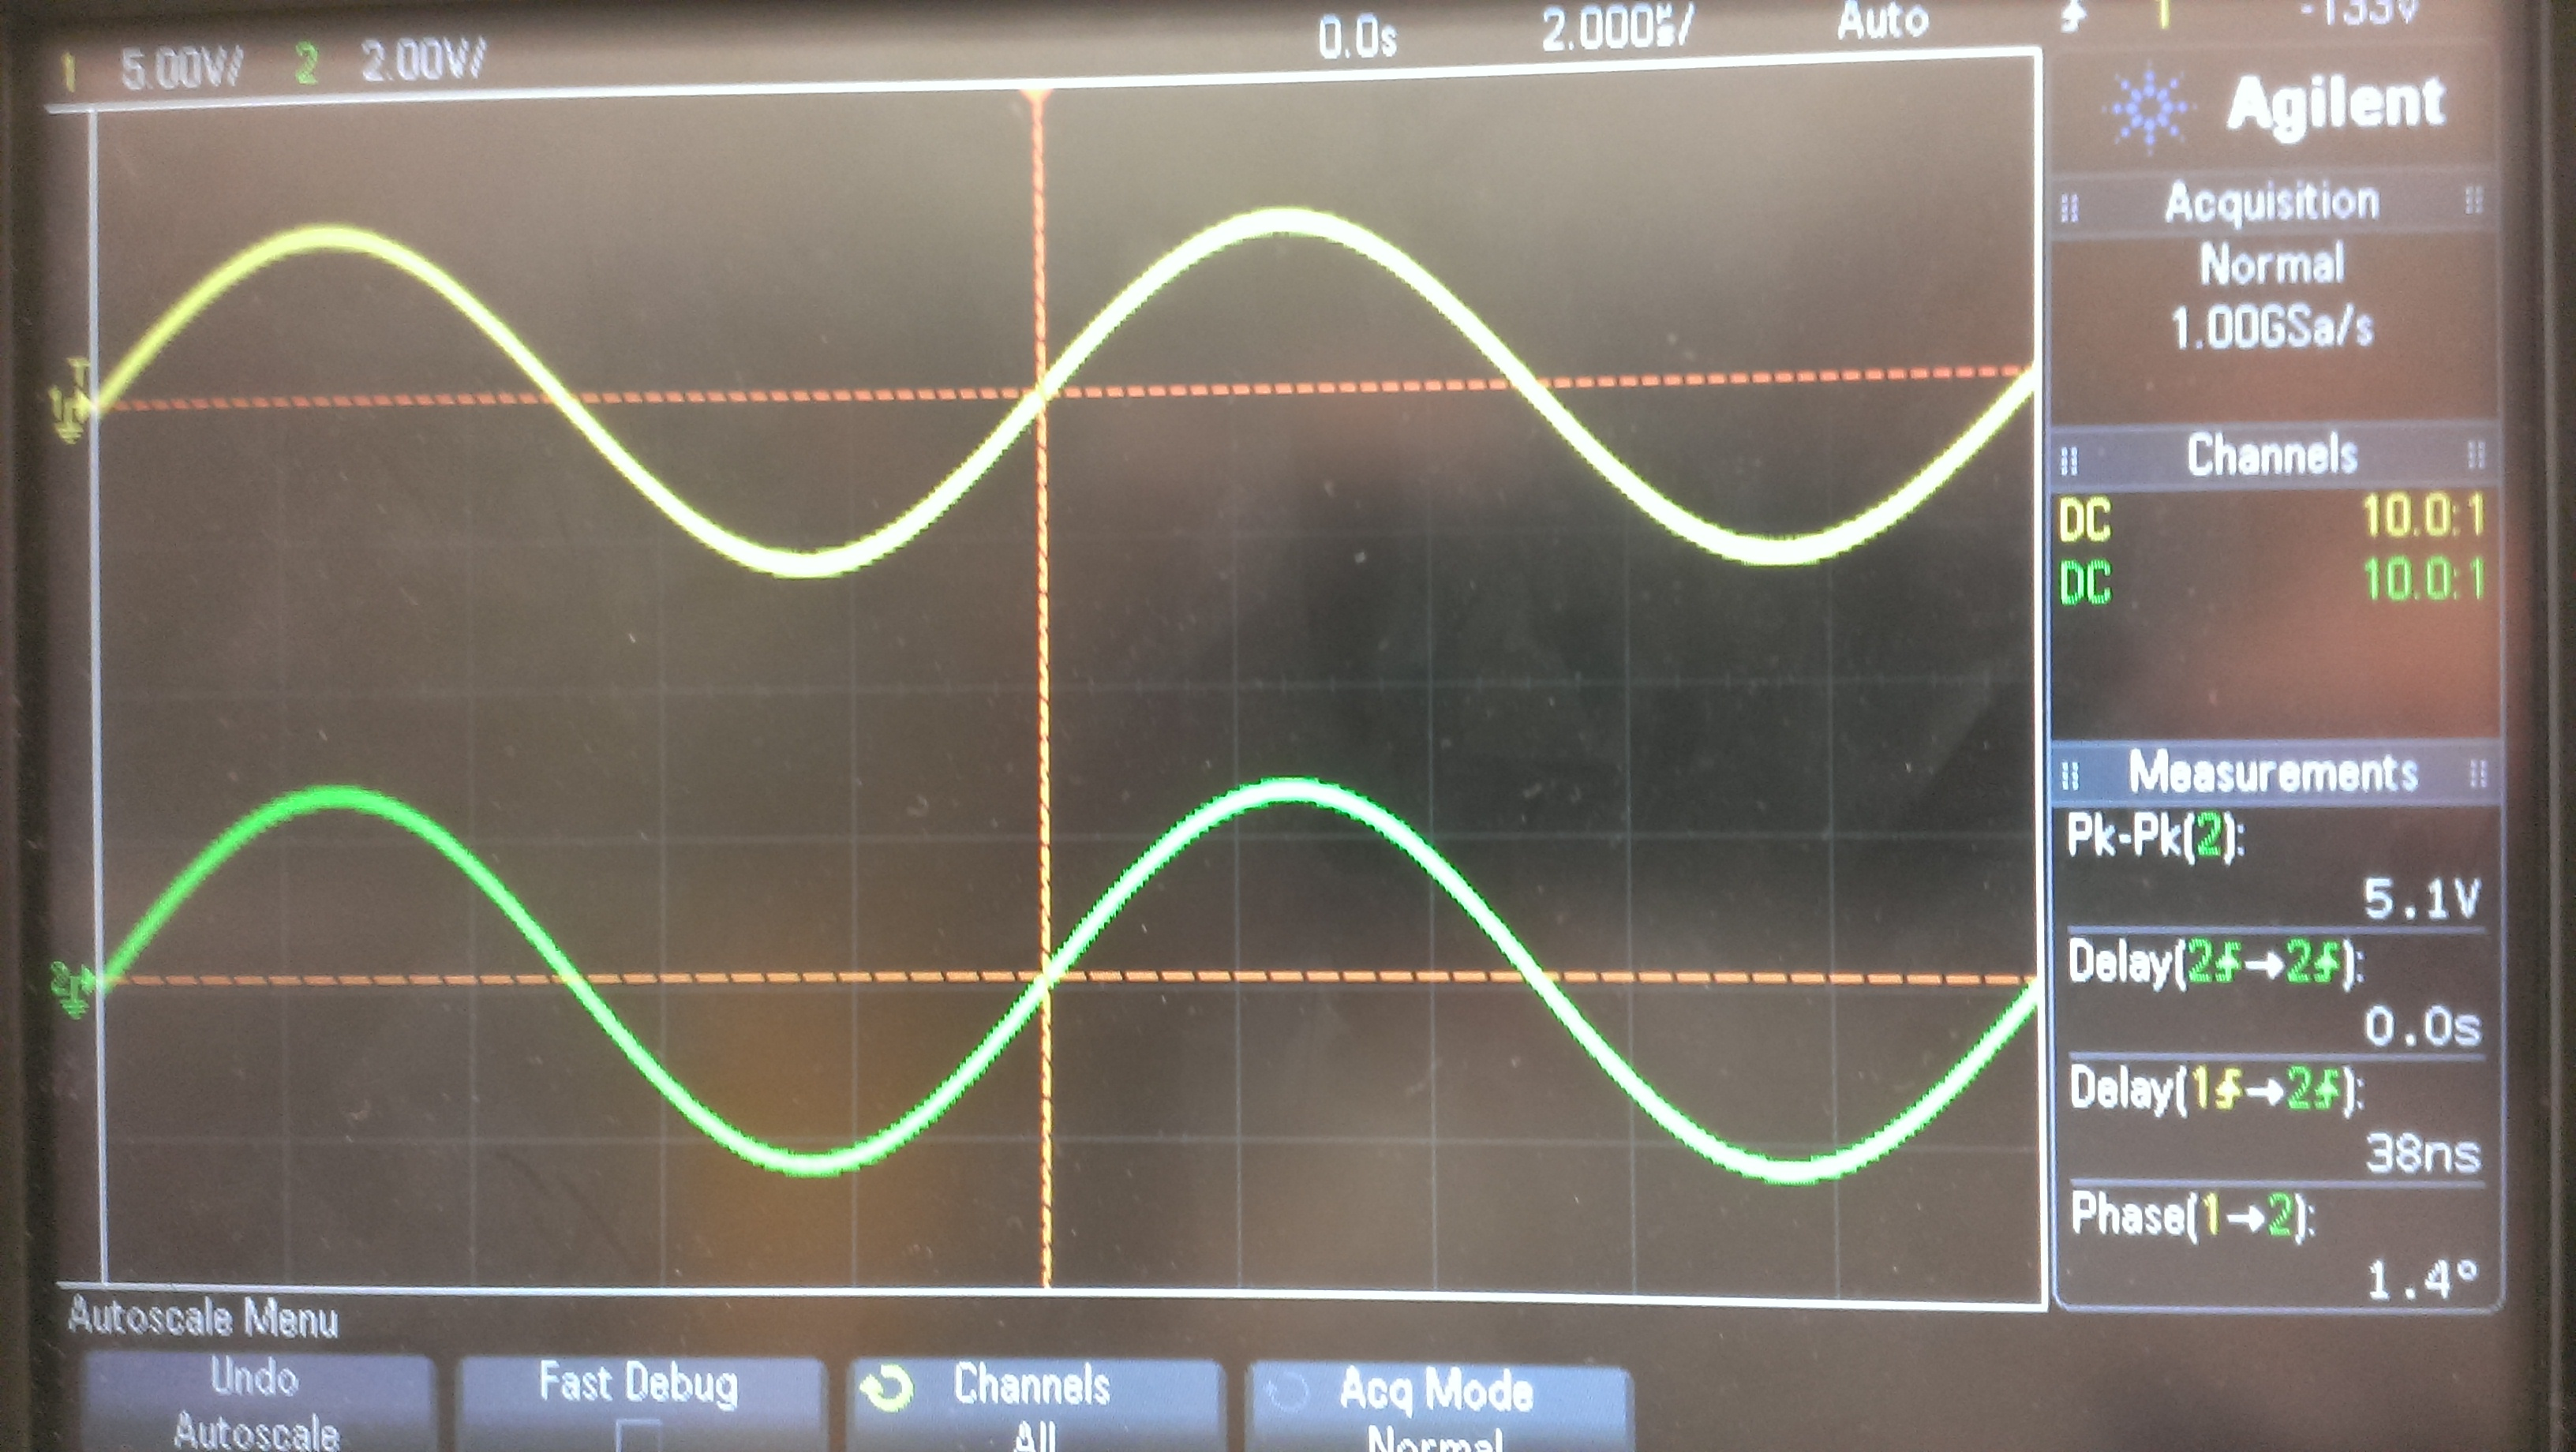
\includegraphics[width=0.8\textwidth]{./Images/RoleWave1.jpg}
    \caption{Oscilloscope output for a 100 kHz signal along a 12" cable}
\end{figure}
\begin{figure}[H]
    \centering
    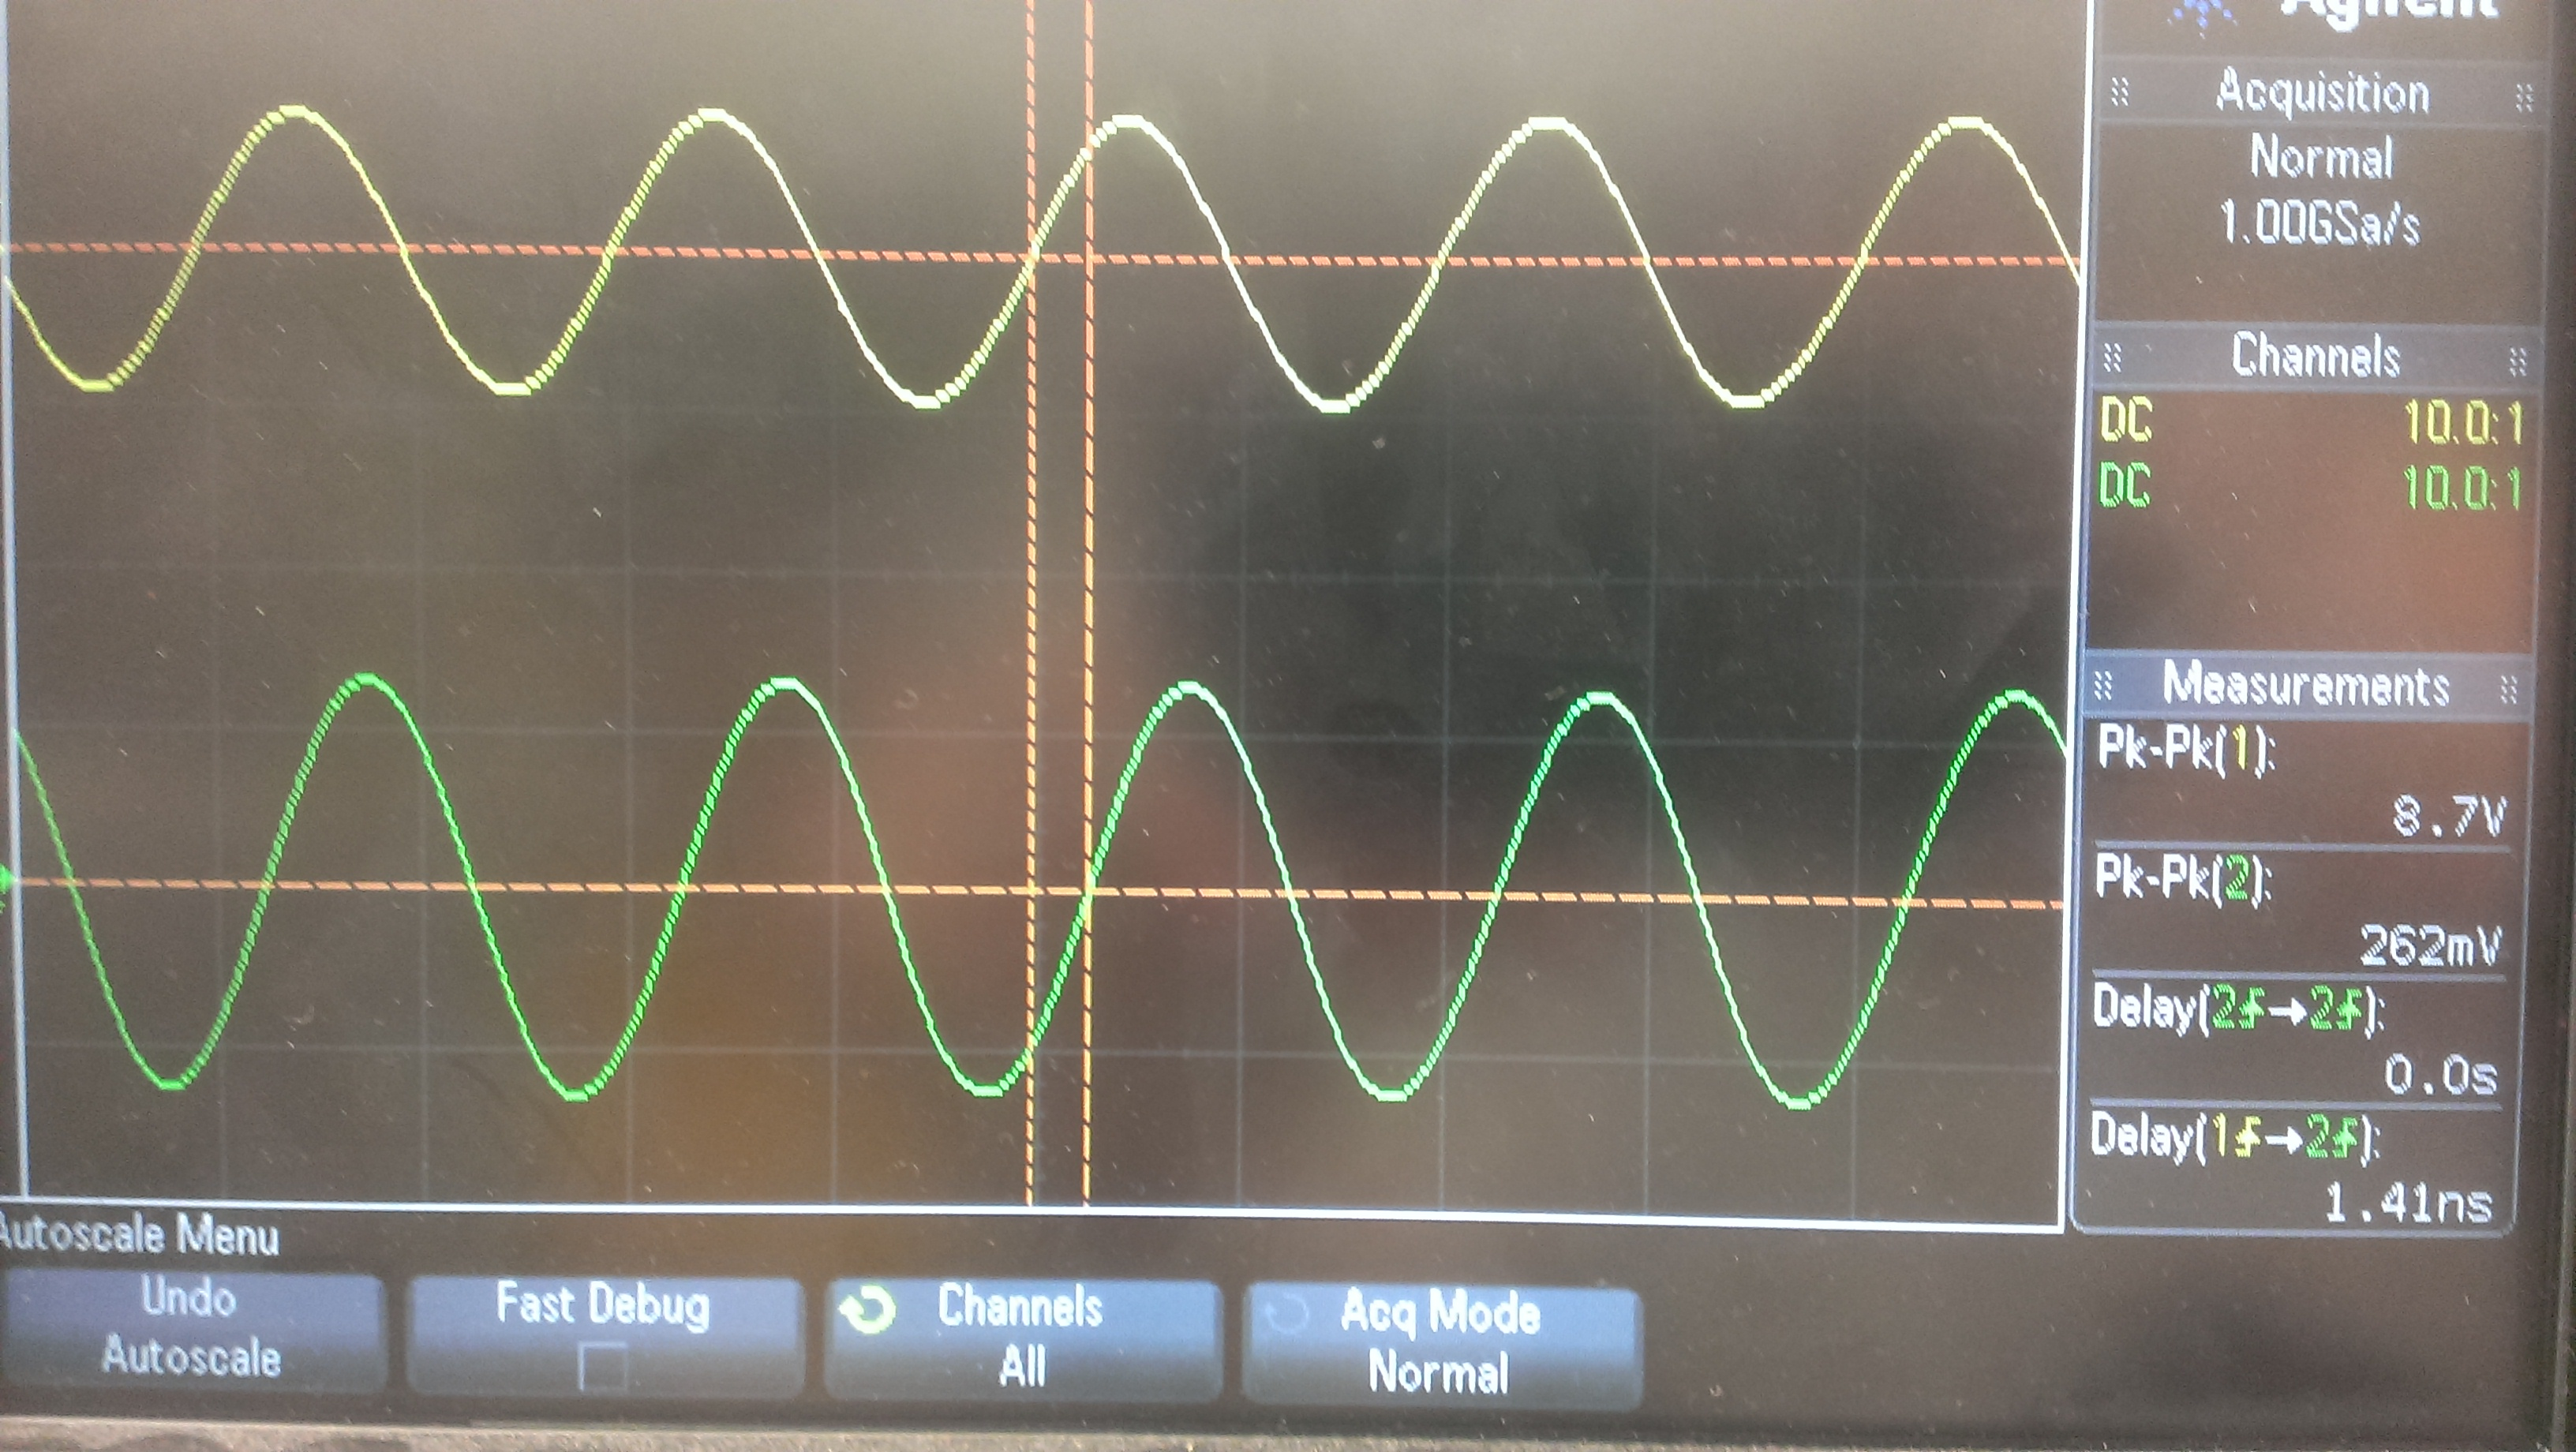
\includegraphics[width=0.8\textwidth]{./Images/RoleWave2.jpg}
    \caption{Oscilloscope output for a 100 kHz signal along a 180" cable}
\end{figure}
\begin{figure}[H]
    \centering
    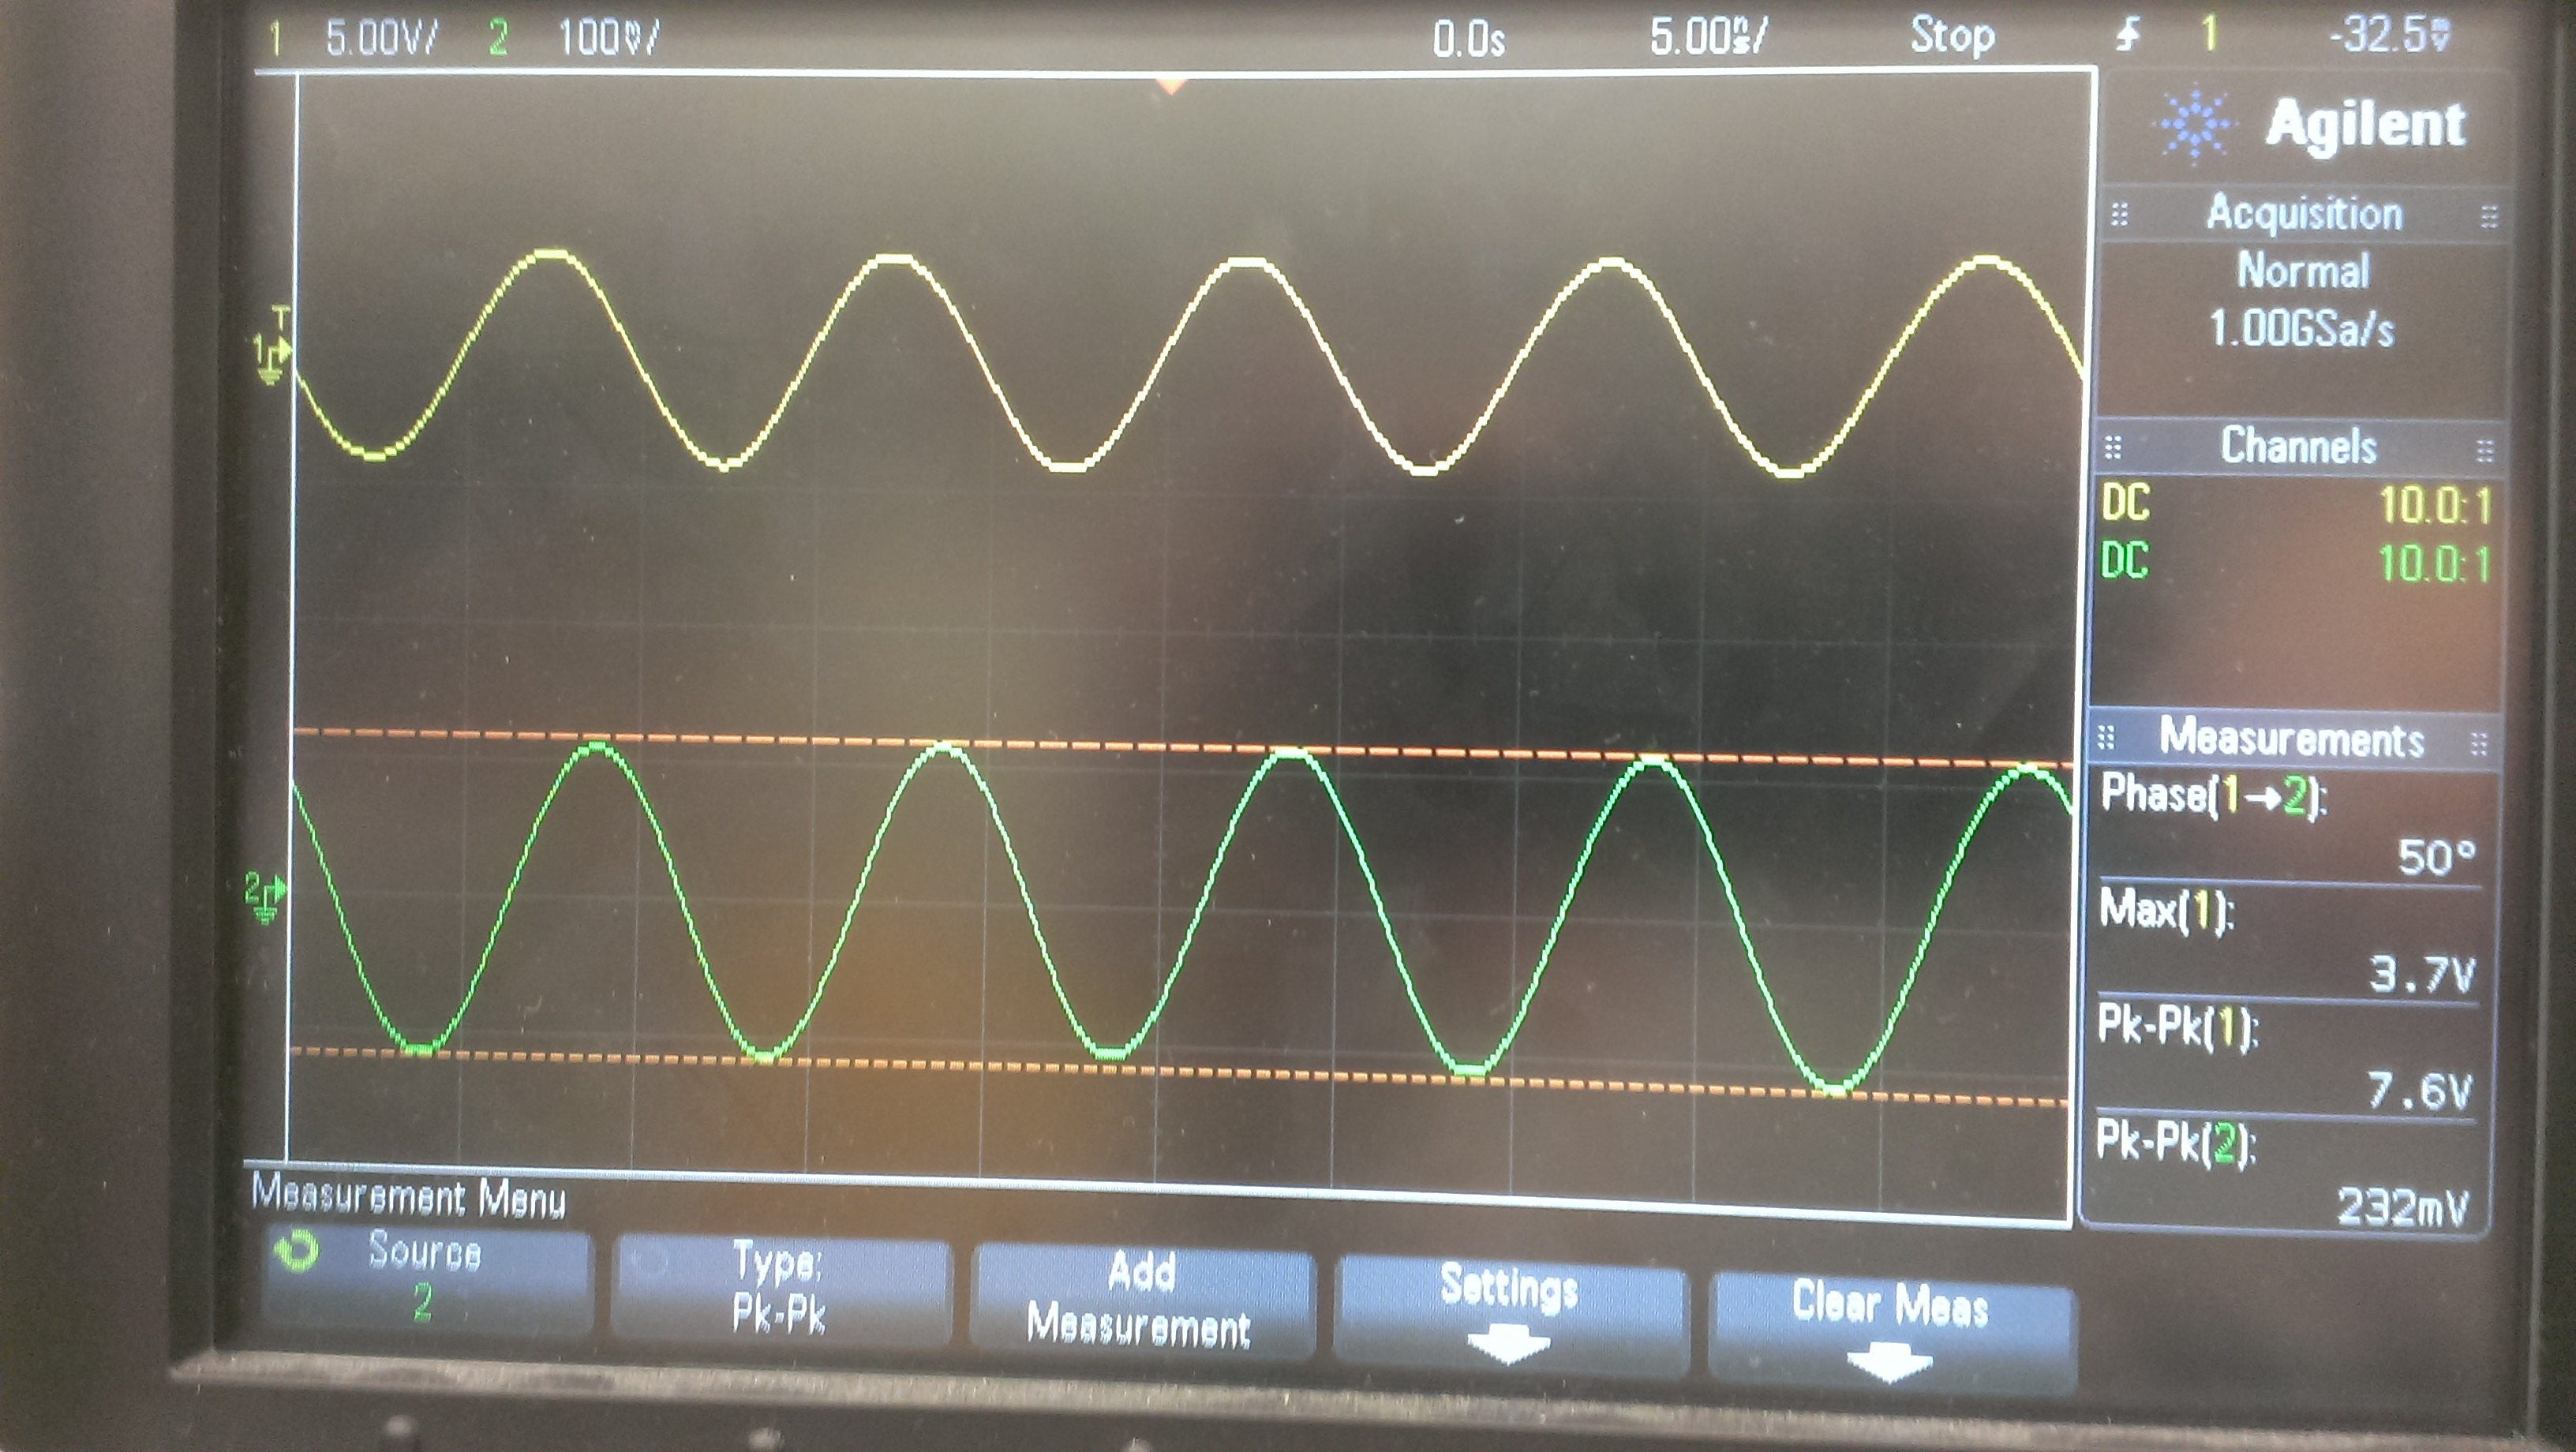
\includegraphics[width=0.8\textwidth]{./Images/RoleWave3.jpg}
    \caption{Oscilloscope output for a 100 MHz signal along a 12" cable}
\end{figure}
\begin{figure}[H]
    \centering
    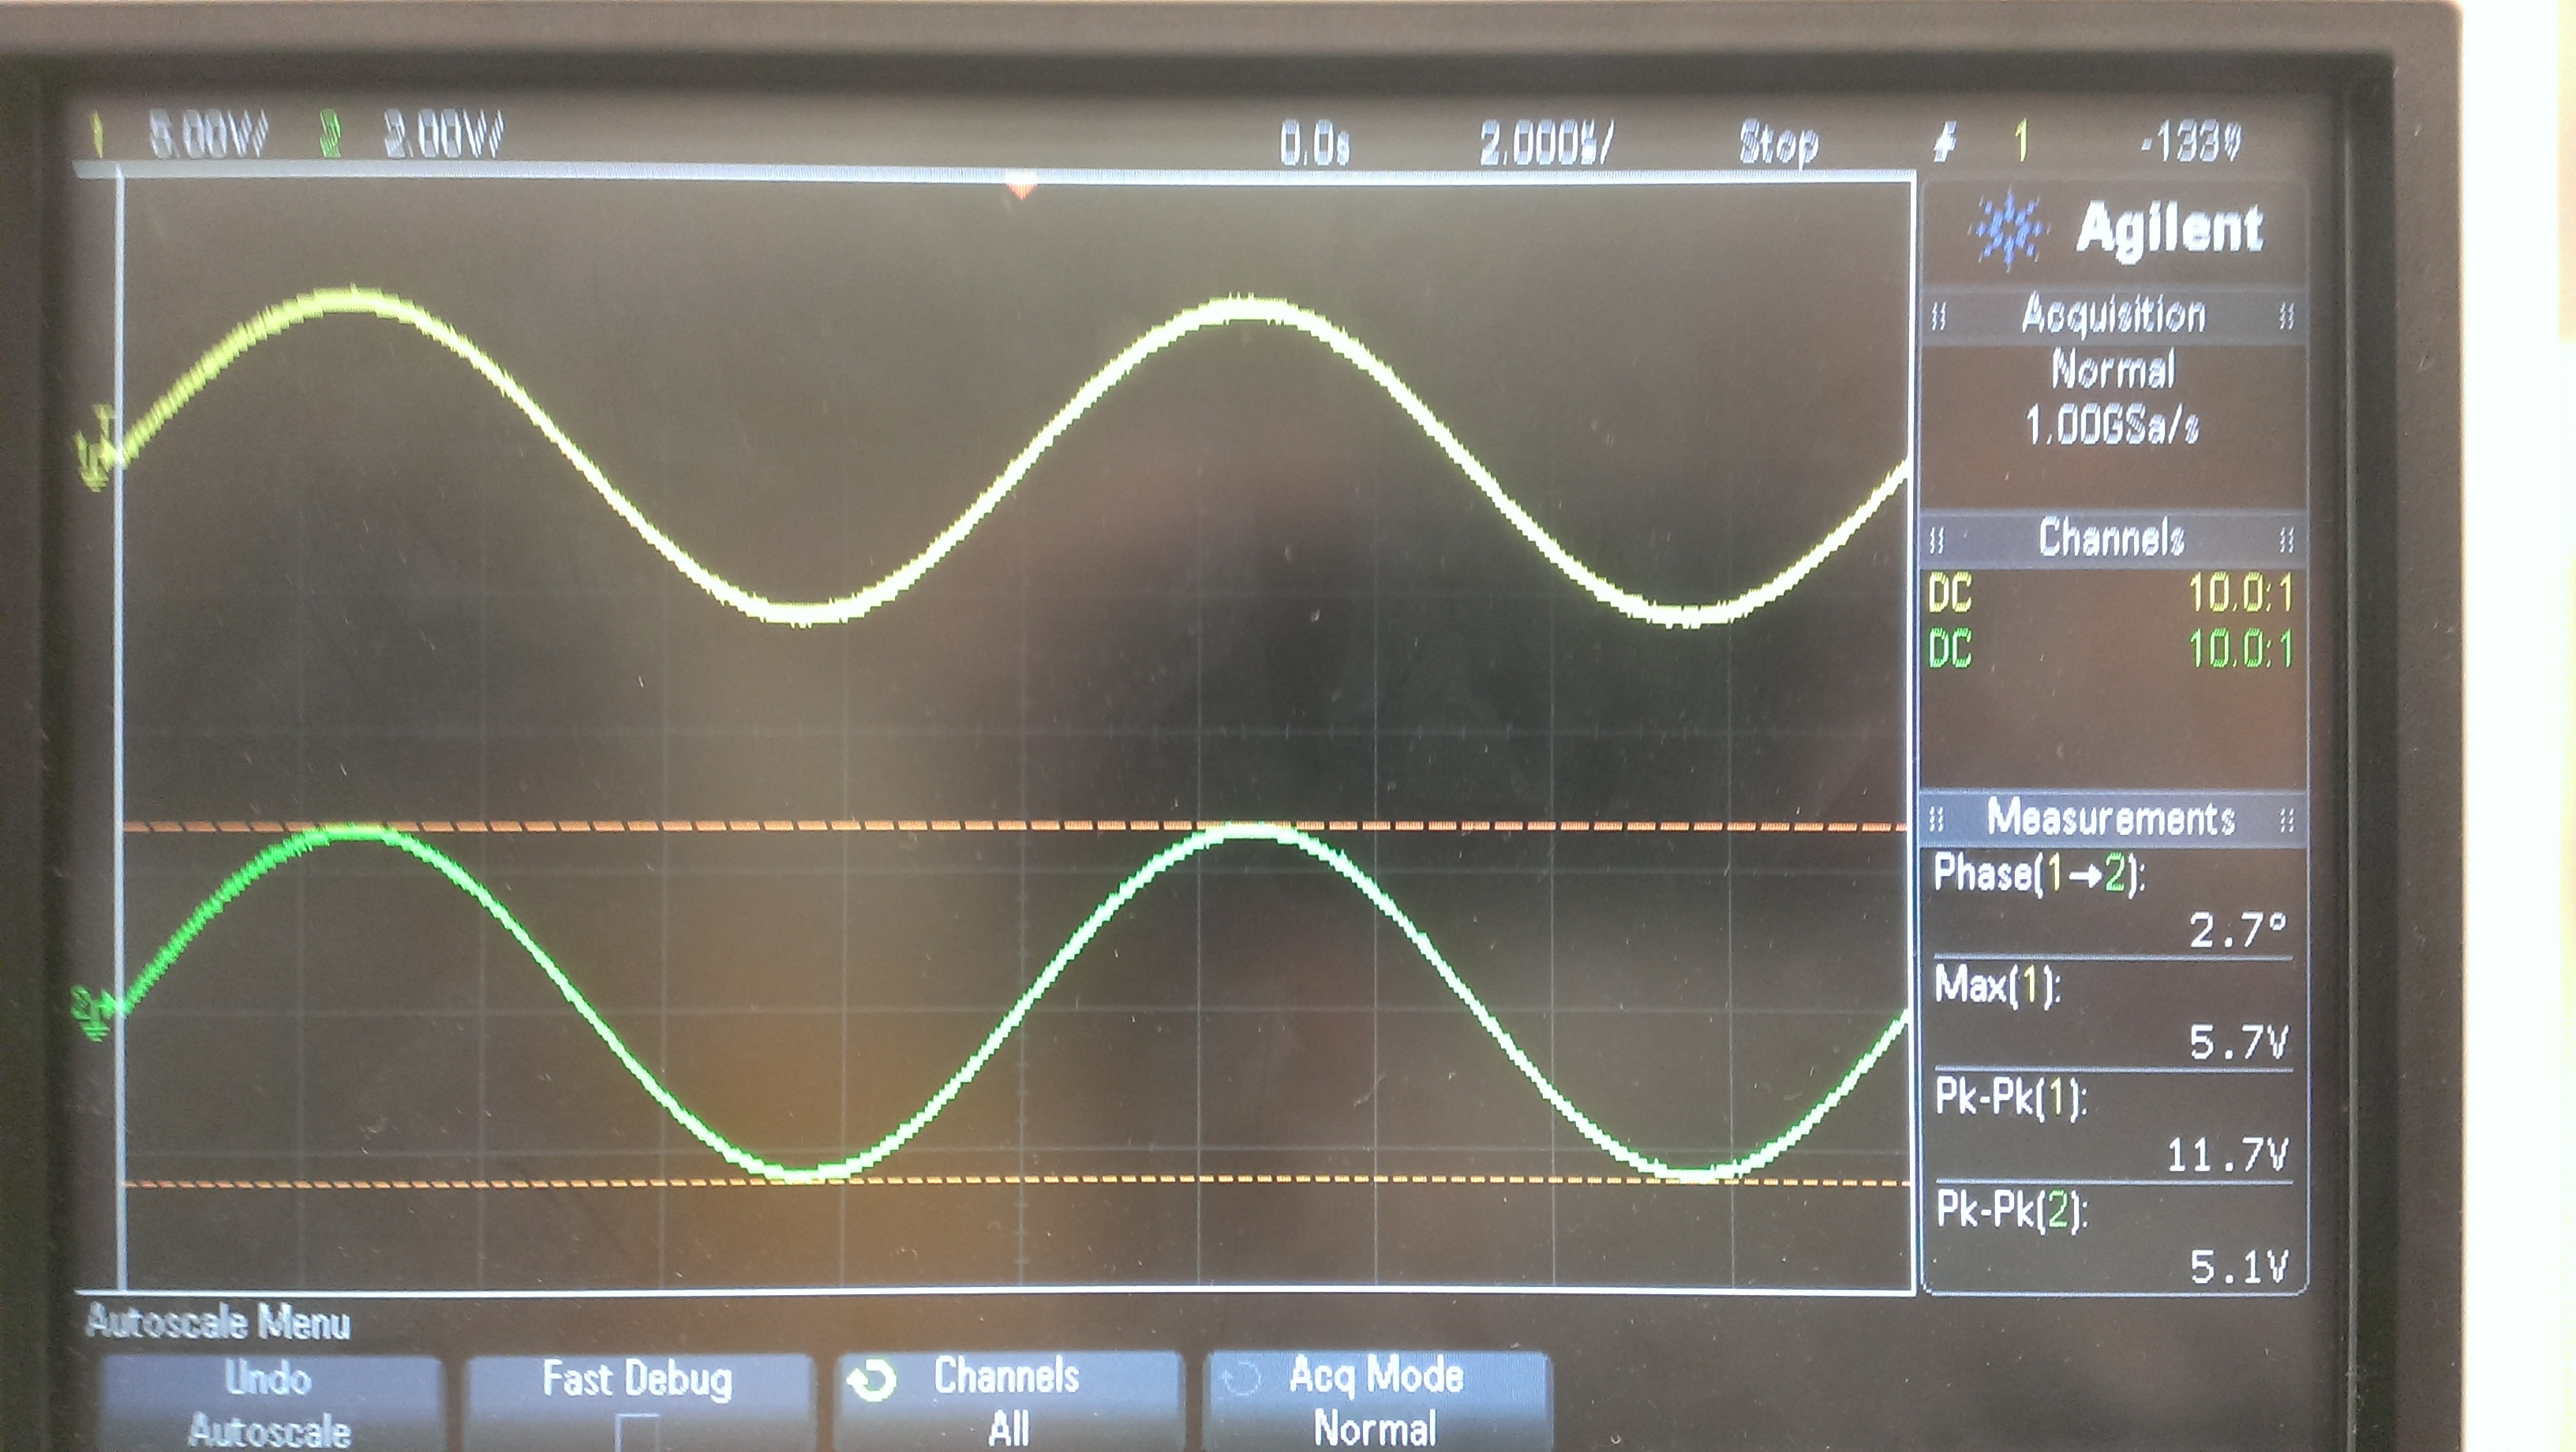
\includegraphics[width=0.8\textwidth]{./Images/RoleWave4.jpg}
    \caption{Oscilloscope output for a 100 MHz signal along a 180" cable}
\end{figure}
\begin{figure}[H]
    \centering
    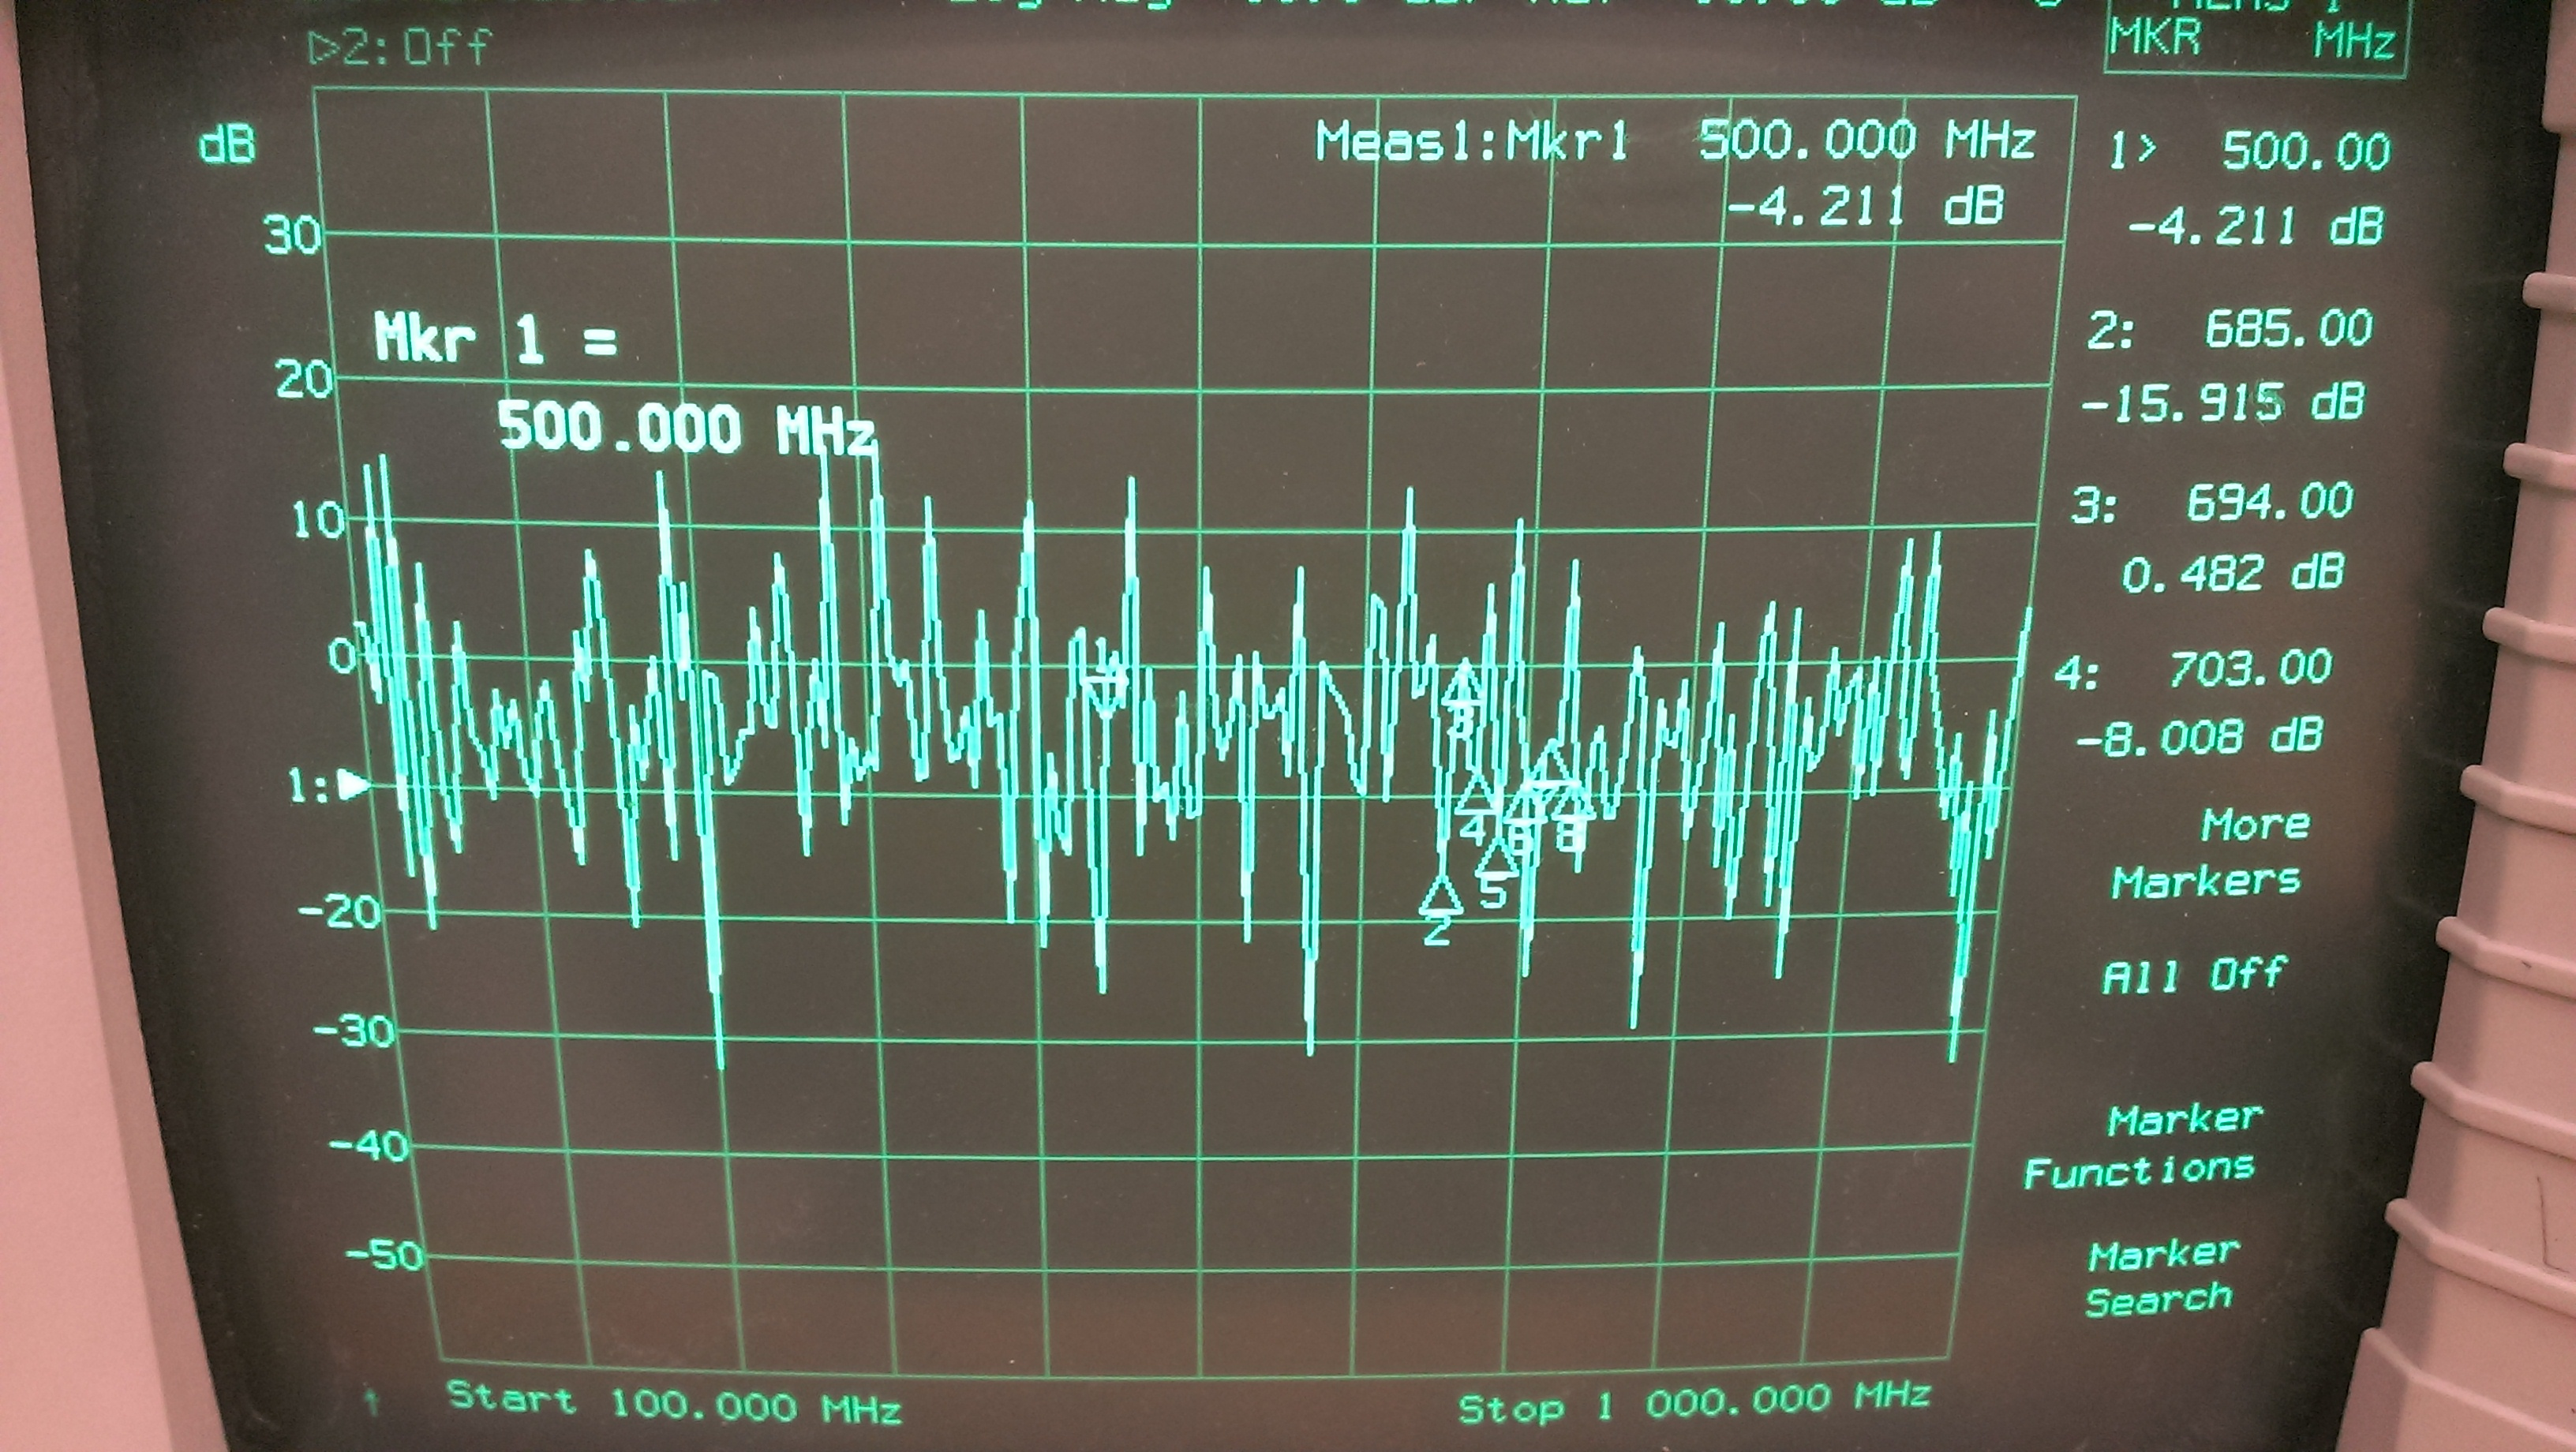
\includegraphics[width=0.8\textwidth]{./Images/NetShortUncal.jpg}
    \caption{Uncalibrated network analyzer output for a shorted load}
\end{figure}
\begin{figure}[H]
    \centering
    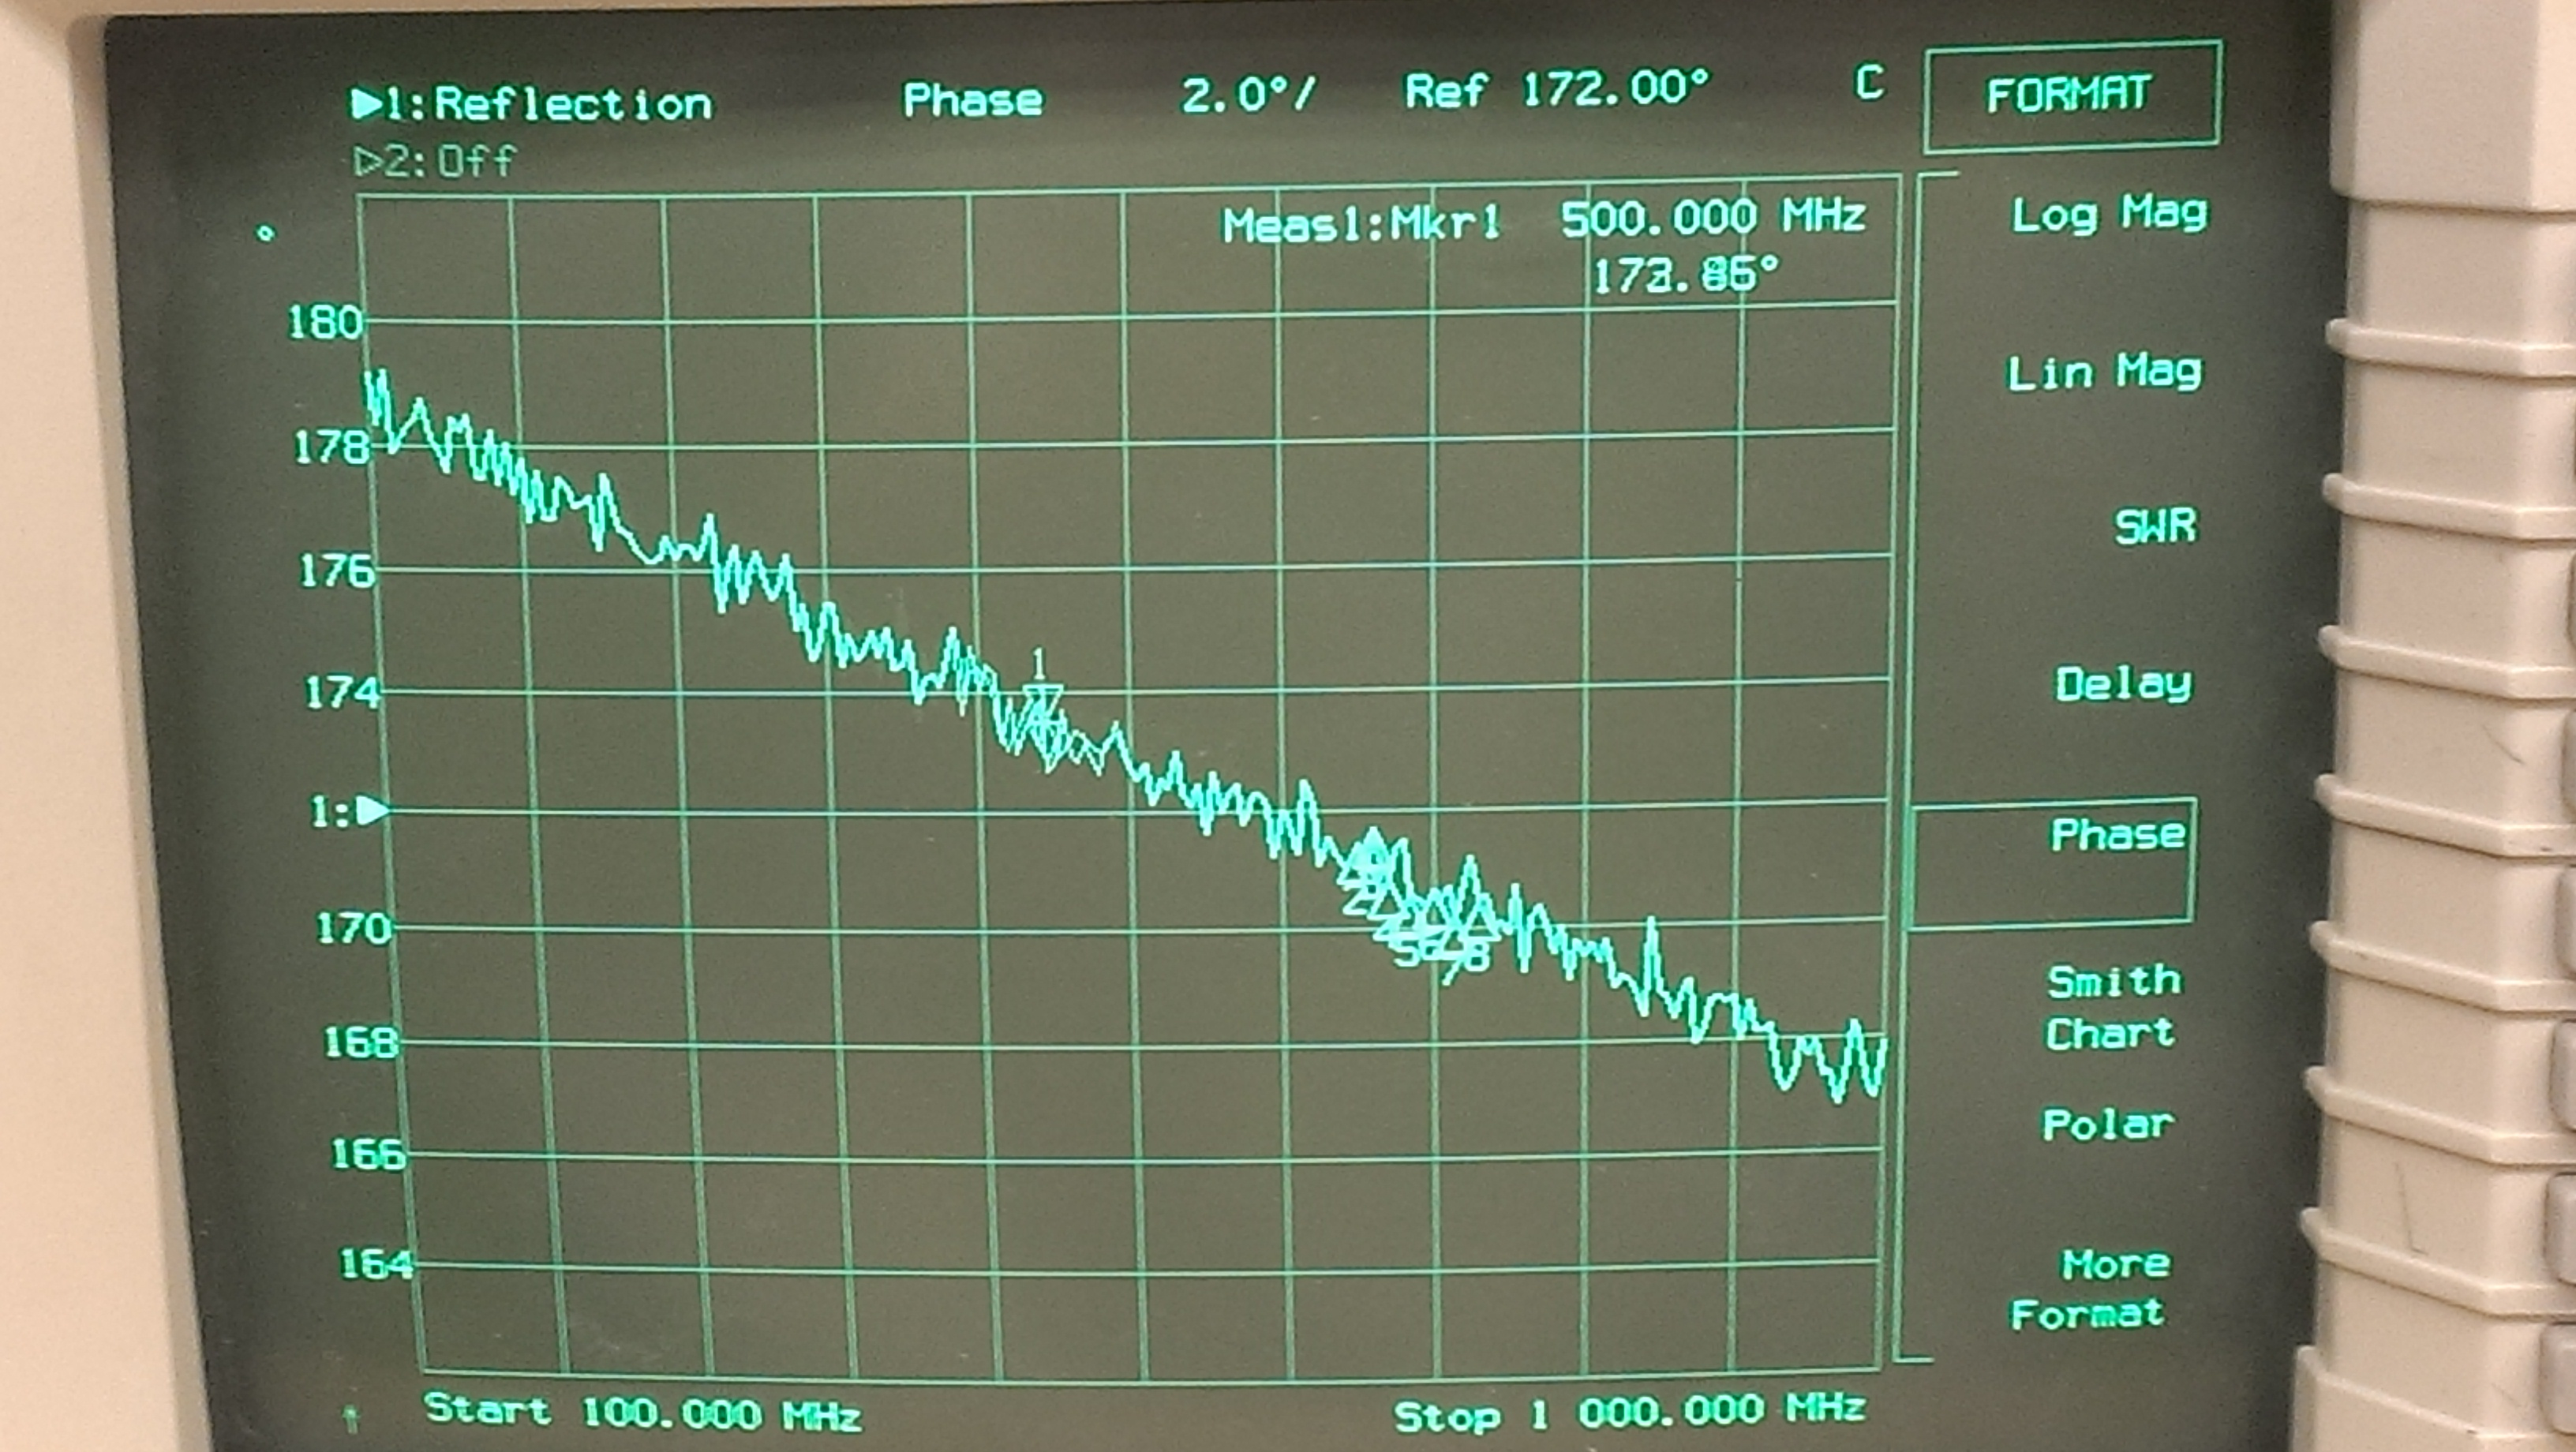
\includegraphics[width=0.8\textwidth]{./Images/NetShortCal.jpg}
    \caption{Calibrated network analyzer output for a shorted load}
\end{figure}
\begin{figure}[H]
    \centering
    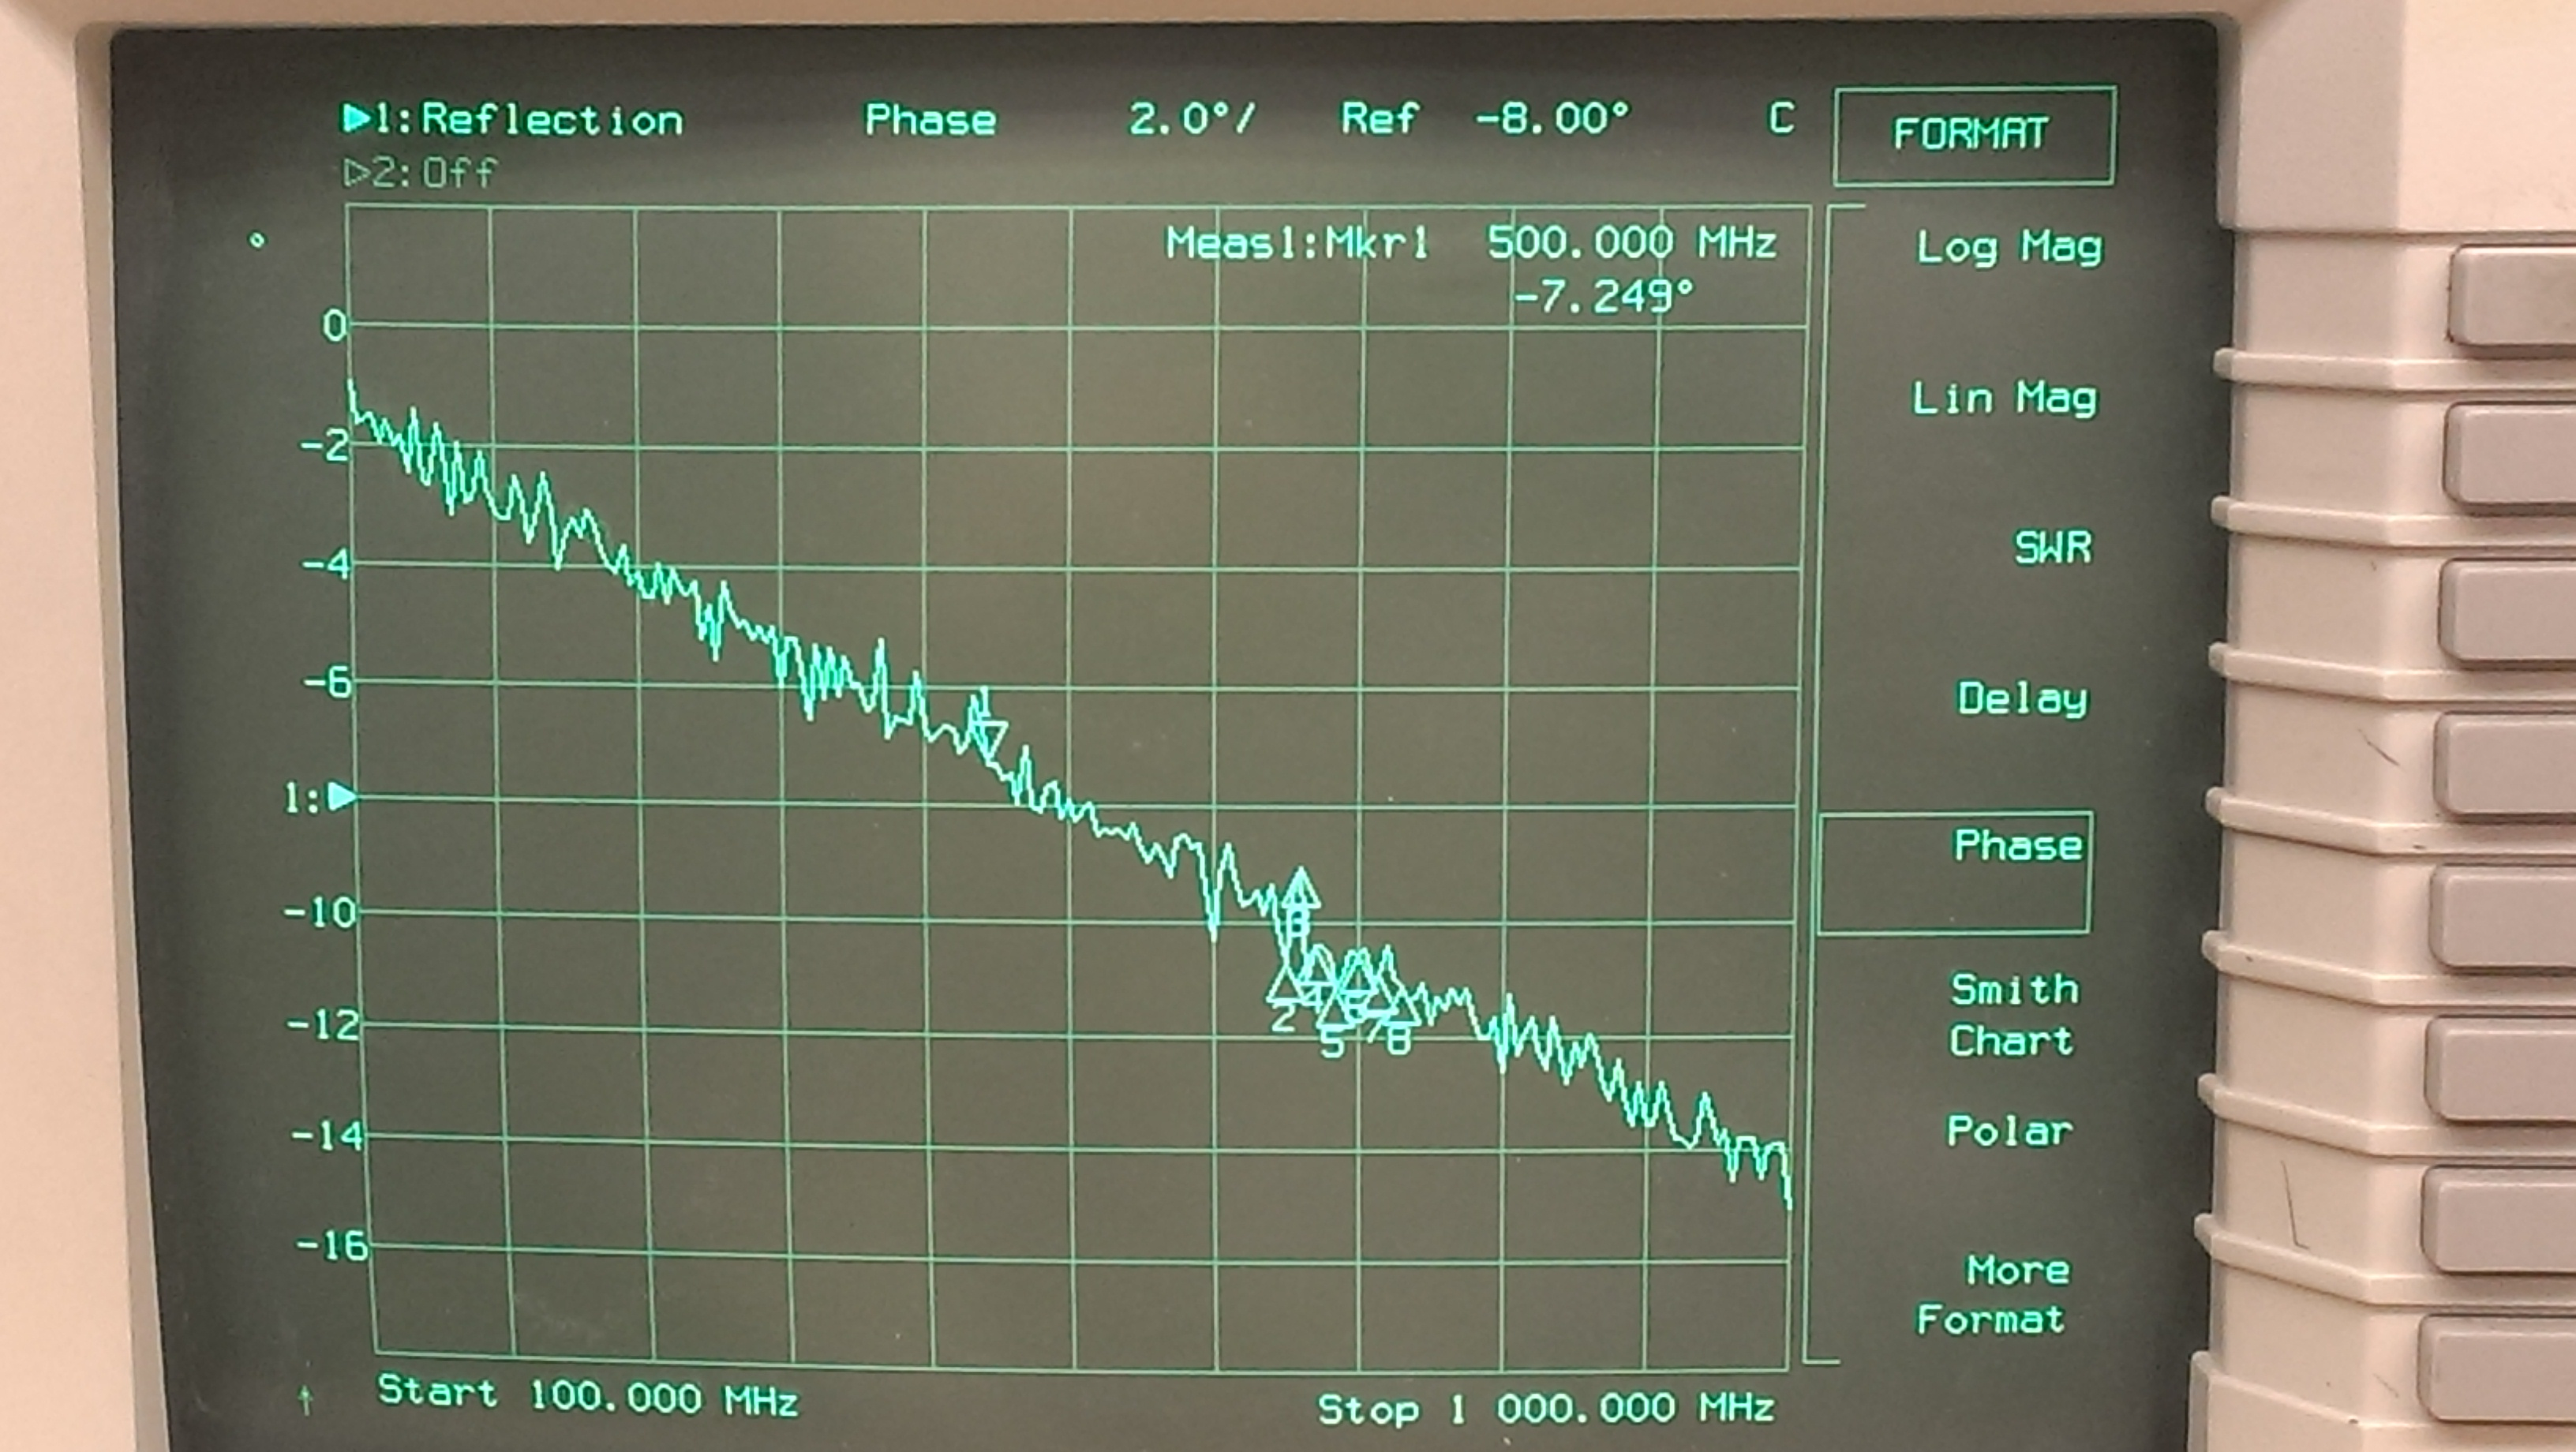
\includegraphics[width=0.8\textwidth]{./Images/NetOpen.jpg}
    \caption{Calibrated network analyzer output for a open load}
\end{figure}
\begin{figure}[H]
    \centering
    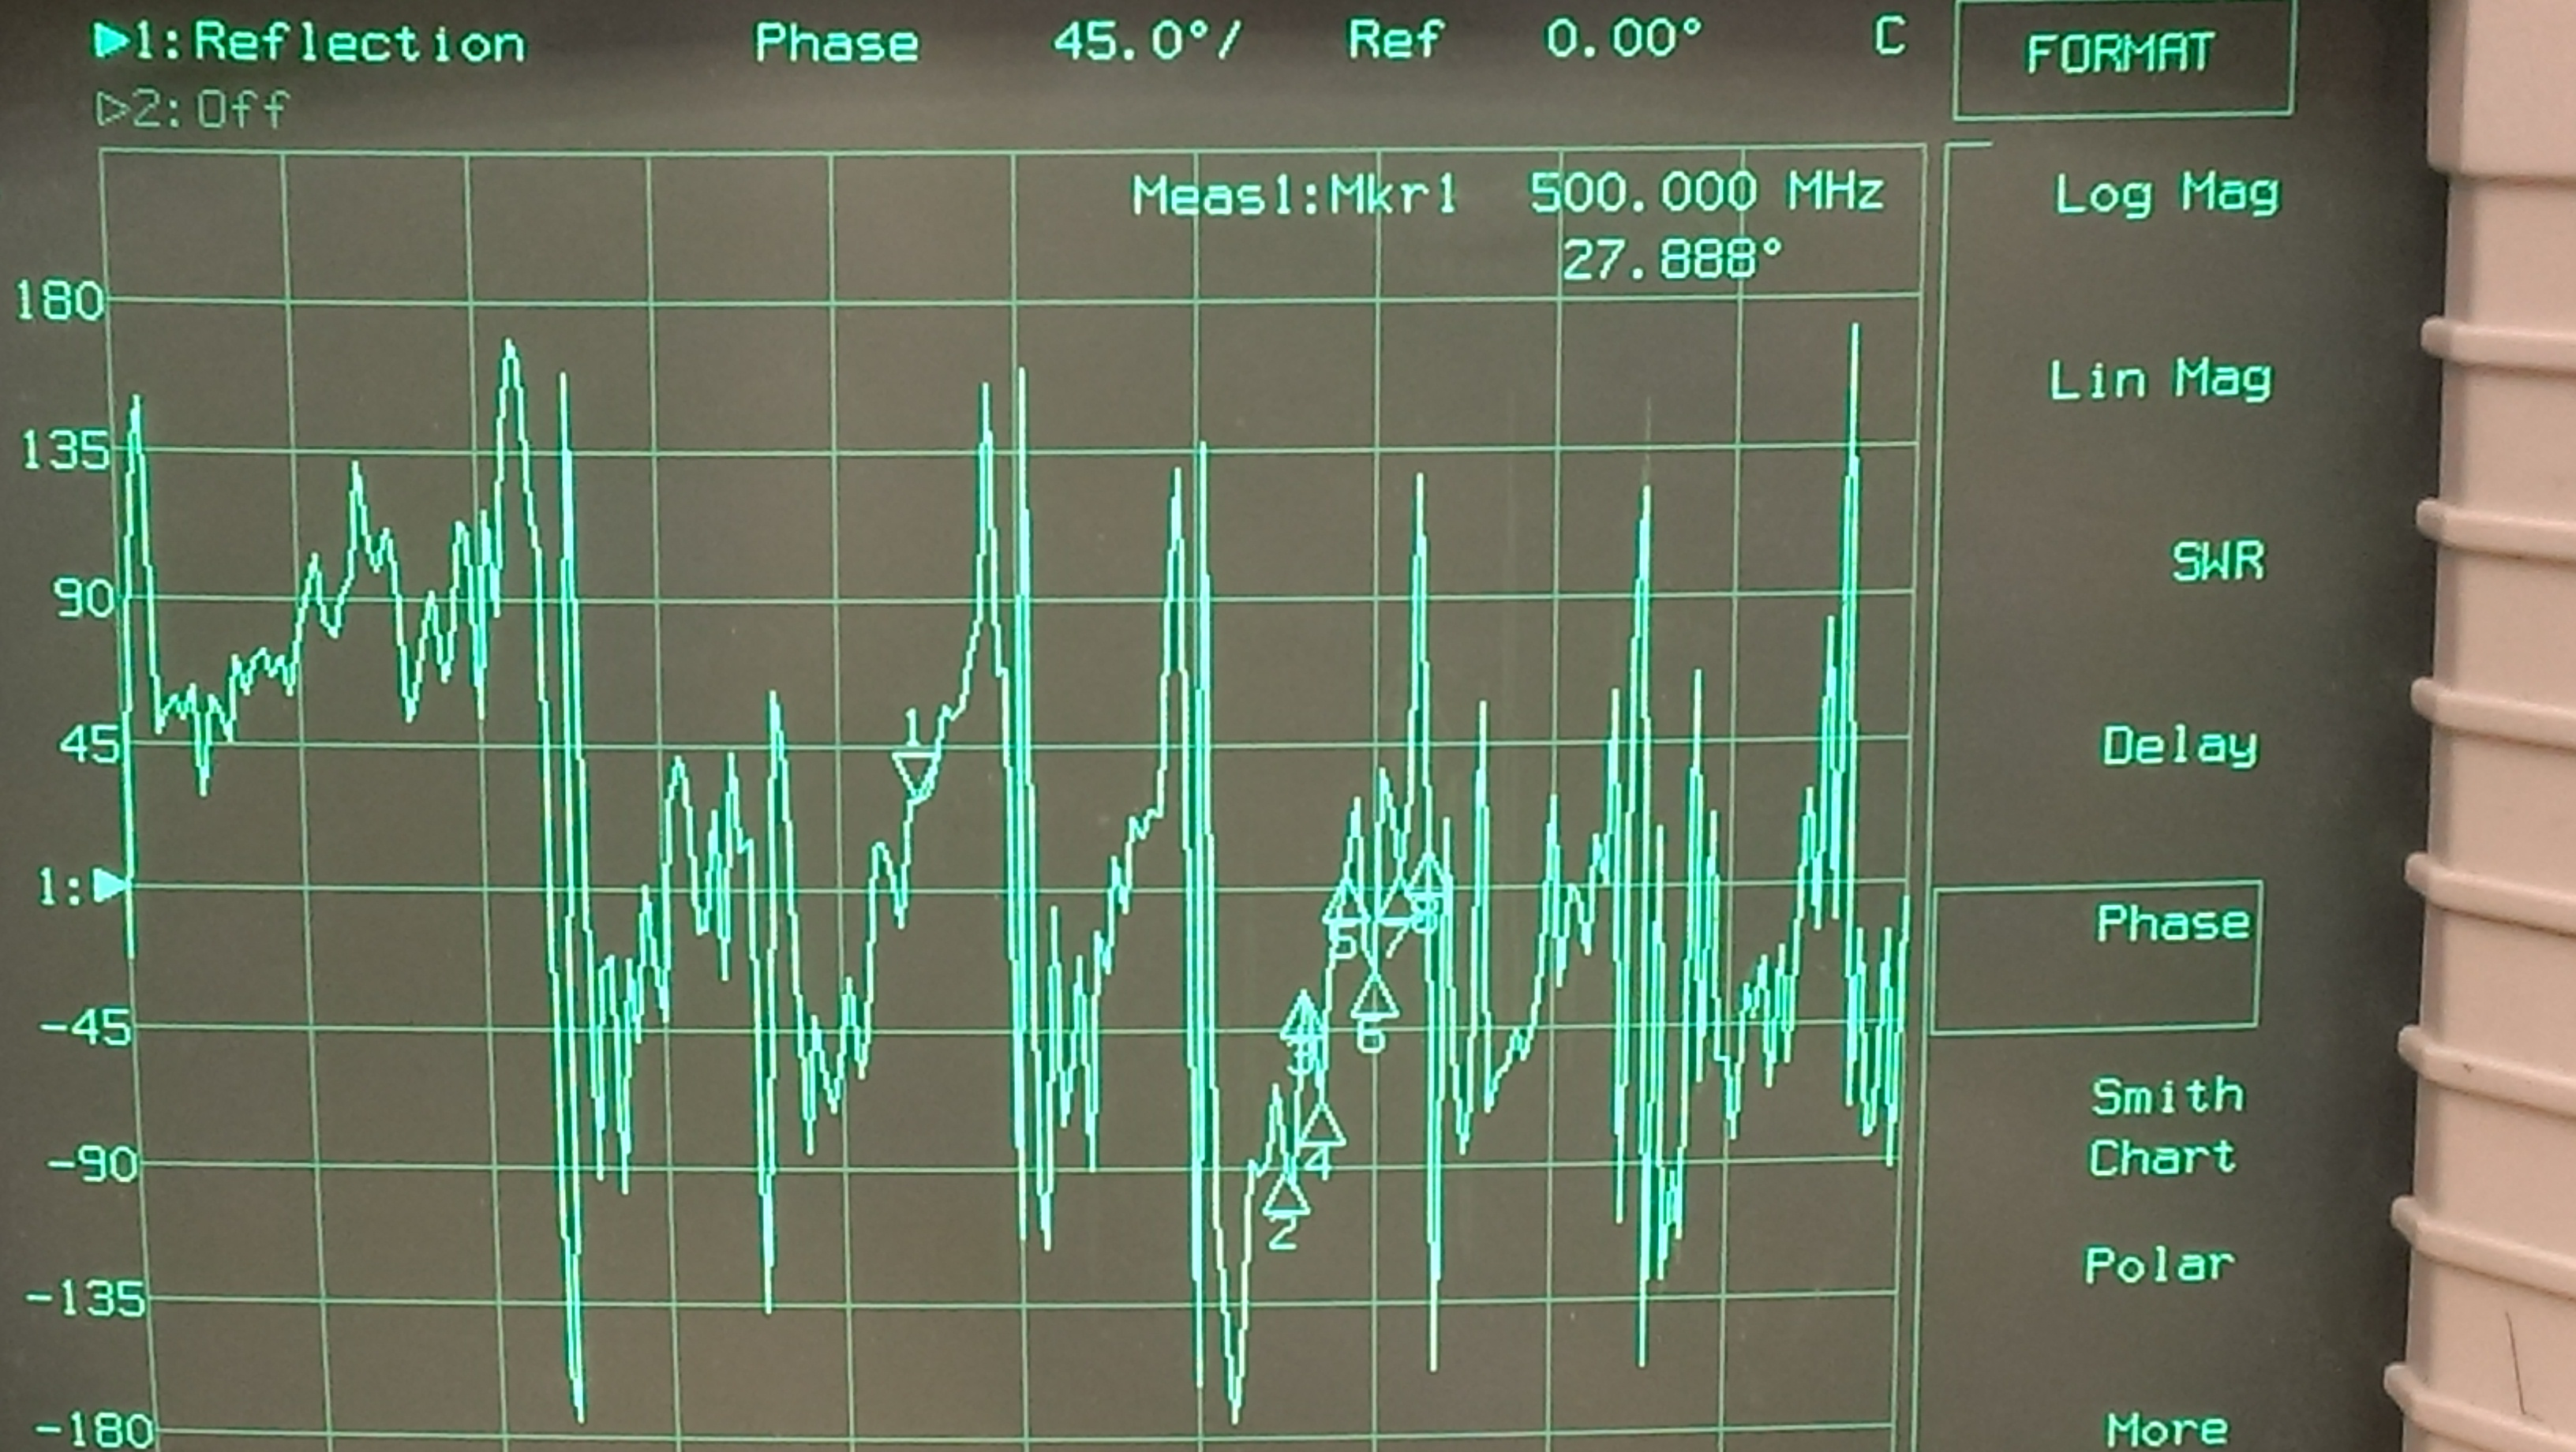
\includegraphics[width=0.8\textwidth]{./Images/NetMatch.jpg}
    \caption{Calibrated network analyzer output for a 50 $\Omega$ matched load}
\end{figure}
\begin{figure}[H]
    \centering
    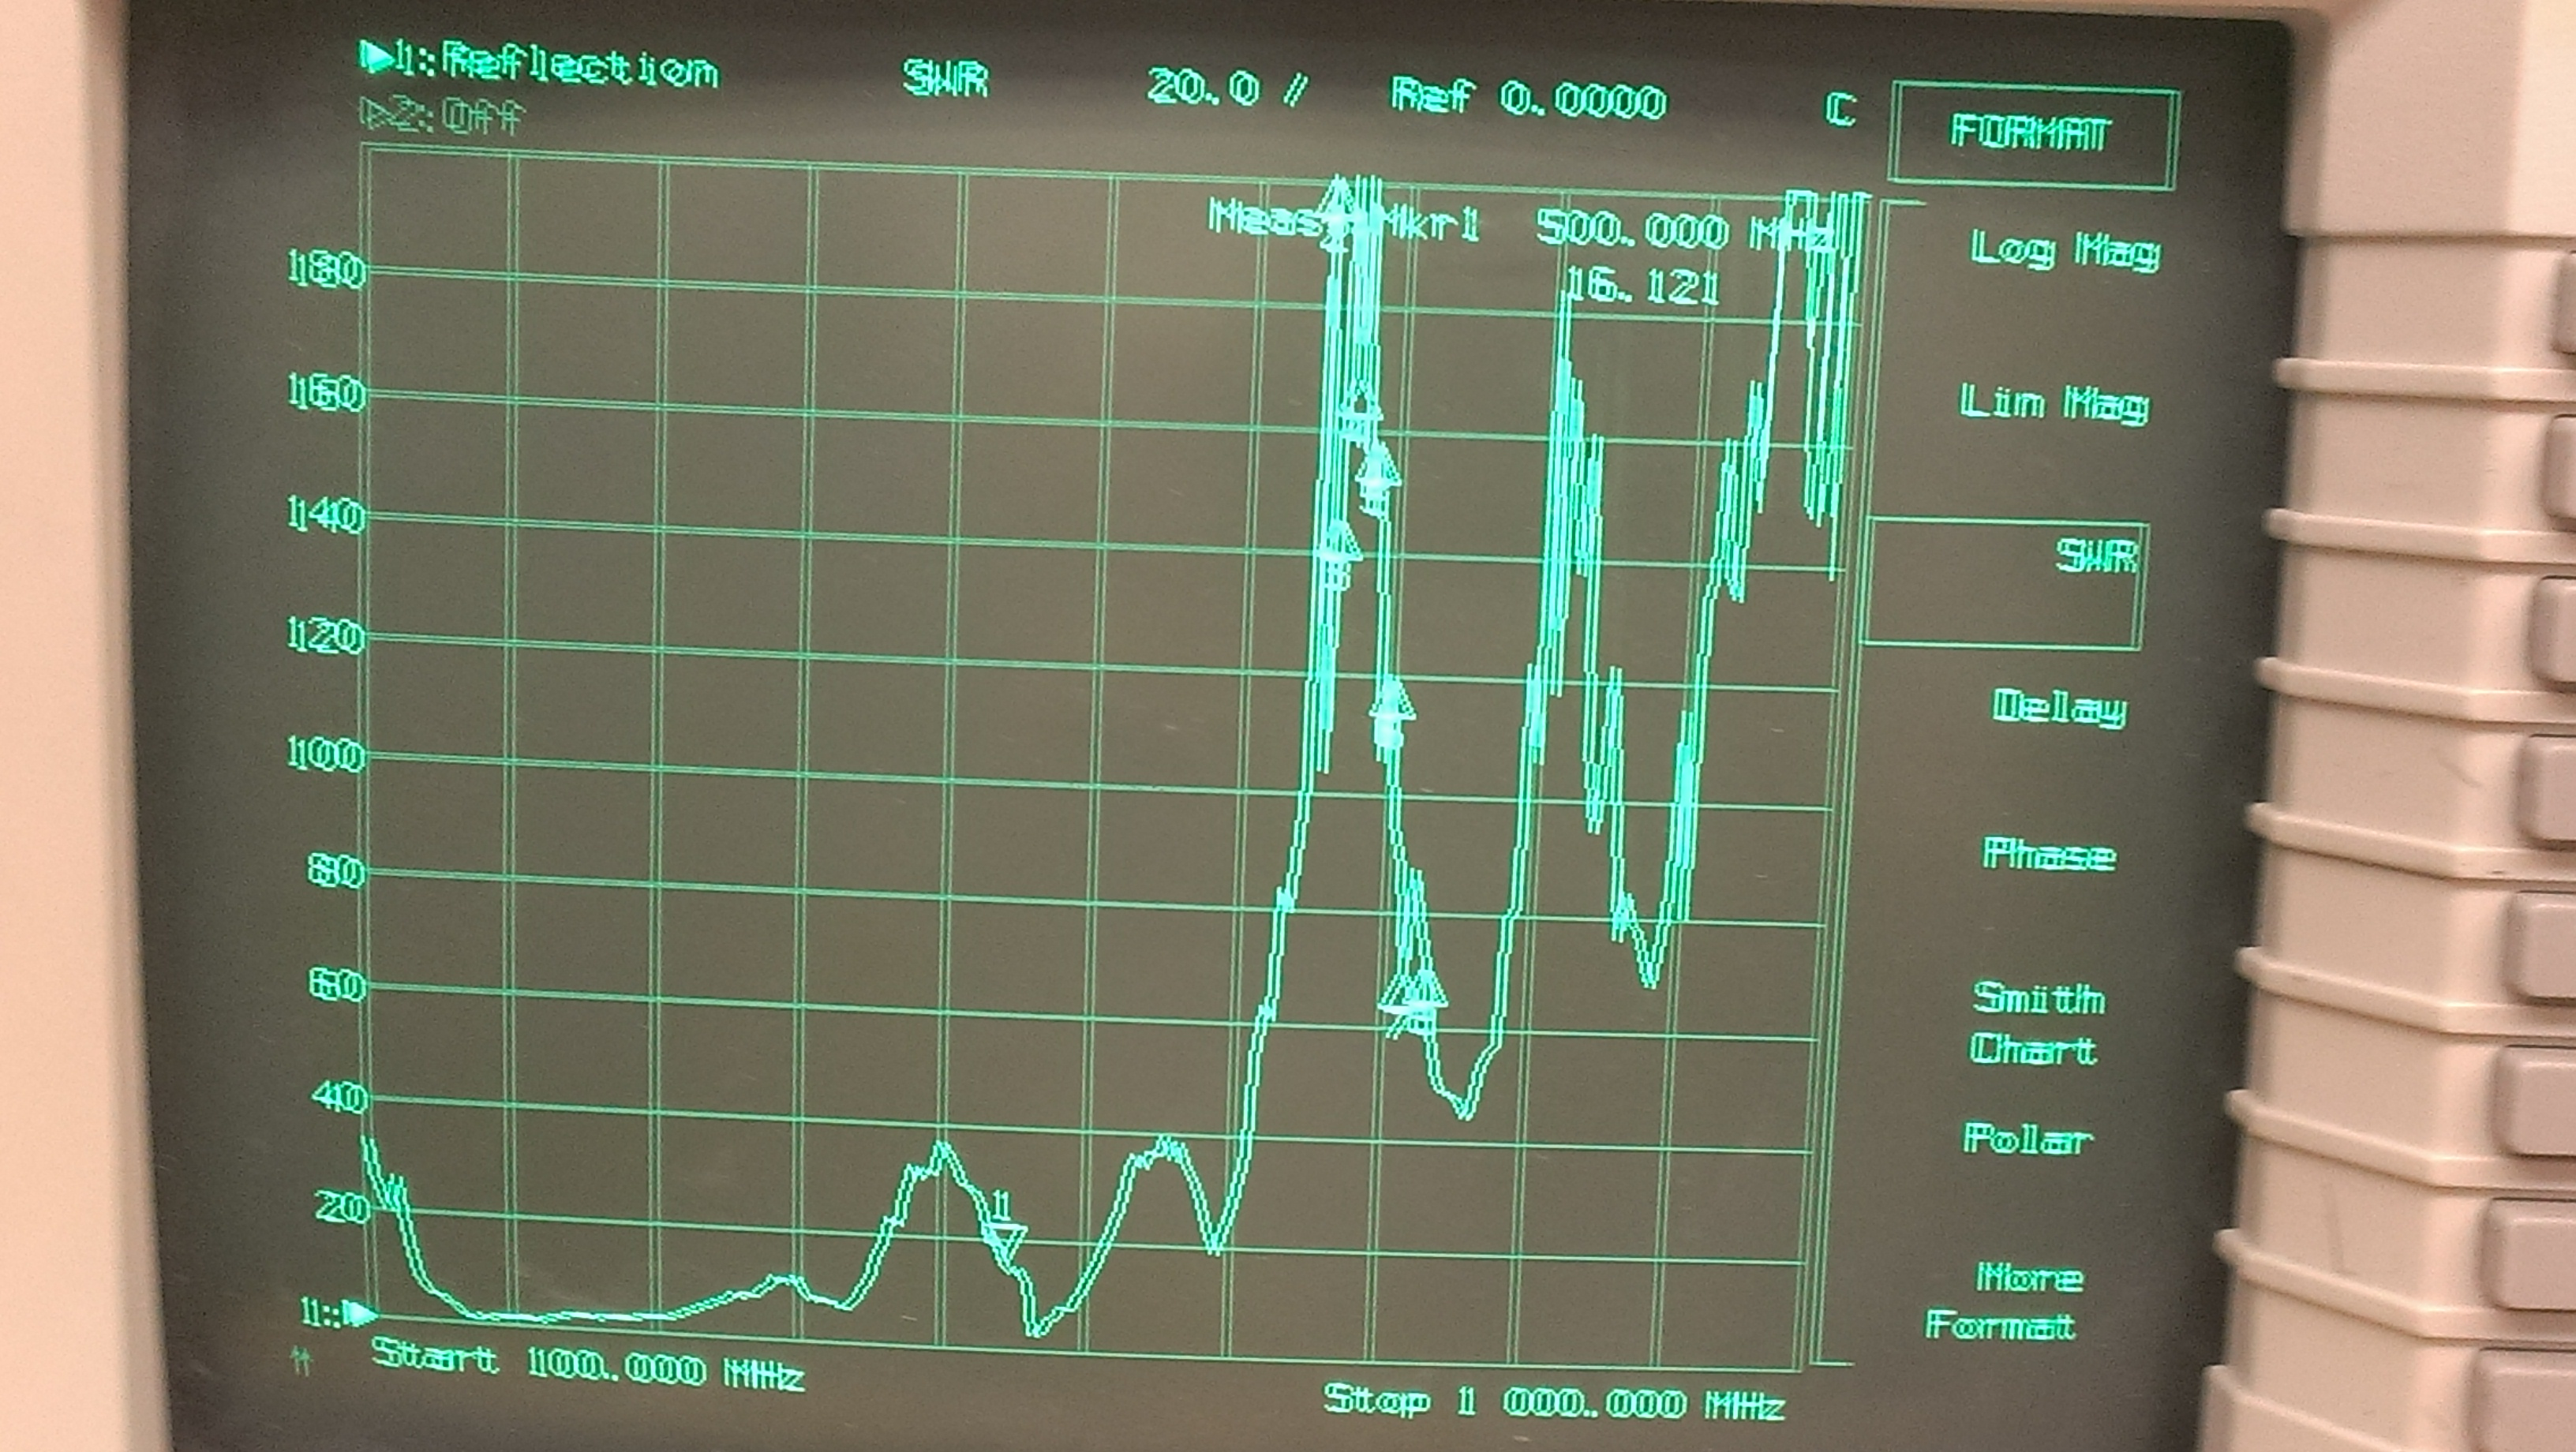
\includegraphics[width=0.8\textwidth]{./Images/NetSWR.jpg}
    \caption{Network analyzer output for the scanner antenna SWR}
\end{figure}

\end{document}
